\chapter{Analysis}
In this chapter we would like to explain the thinking process before and during the implementation of the back-end application. We are going through individual parts from the back-end application requirements, explaining problems associated with them and revealing what possibilities we had to solve them and how we decided in the end.

\section{General problems}
\subsection{Authentication}
In our application we had to deal with authentication for customers and employees. There are many ways how users can be authenticated in API. We ended up with token authentication - in each request clients must set the Authorization header with the token. Client can get the token in exchange for correct credentials.

Another part of the authentication we consider in the analysis is at least the basic security during the manipulation with auth data and flawless verifying token sending.

\subsubsection{Token authentication details}

We decided to implement it on our own, using only Rails helpers for generating and verifying secure tokens. As you can see in \ref{auth-token-scheme}, token is generated during the login action and then returned in body of the response. All the following requests must have this token in it's header to be authenticated.

\begin{figure}[h]\centering
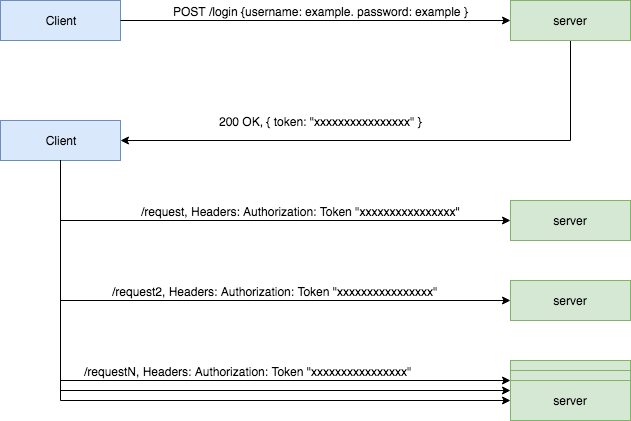
\includegraphics[width=\textwidth]{auth/Auth.png} 
\caption{Auth token scheme}\label{auth-token-scheme}
\end{figure}

Our application store just one token per user. That implies the user can be logged in from one device at time only. Having more valid token for users would let into several problems with invalidating them in case of log out and also this approach has one advantage. If someone reveals user credentials and log in with them - user will know that in the moment it tries to use the app, because all it's requests would be unauthenticated.

In Ruby on Rails there exists very good gem for authentication - \textit{devise\_token\_auth} \footnote{\url{https://github.com/lynndylanhurley/devise\_token\_auth}} which we half-implemented at first. However we decided to not use it in the end. Main reason for not using it was - at the time of writing the authentication part - very unstable and badly documented front-end library part. More details about problems we came across during the analysis/implementation in the next paragraph.

First reason for not using the gem was, that it uses email as main default authentication field. For customers we wanted to use the telephone number as the main identifier - including the SMS confirmation and password recovery (explained later), which would led us to rewrite the most of the gem's controllers and models anyway and as bonus we would have to integrate it with the existing parts of gem.

Second reason was the complexity of the whole authentication process. This gem would bring more secure but also much more complex way of authenticating to our project. Once the client gets the token from the login endpoint, a new token is generated and returned with each following request. Using this approach we also have to solve the batch request problem. Imagine that the client sends three requests to the server at once. Of course all of the three requests must have the same authentication token - because the client doesn't have the new token until the response arrives. Thus the server must accept all of those three requests as authenticated. Besides that they also must agree which response has the correct new auth token - responses don't have to come in order in which they were sent. This complicated process was implemented in the back-end gem and couldn't be easily changed. The front-end part of the library seemed to be implemented, but after the three weeks of trying and founding several bugs in the library - even without successful login - we gave up using it.

In conclusion if we had wanted to use the gem on backend we would have to understand the whole gem auth process in detail and specify it for the front-end. Front-end would then have to write the whole complicated solution on their own. 

We came to conclusion that the complexity, that would bring this library to our application is not worth the better security and stability we would gain from this. Using HTTPS on both server and client makes the token theft little bit harder - so lack of this generation process with each request is not a big deal. Also the only really sensitive accounts for identity theft are the employees one's and we are in personal contact with them, so we would know about misuse or potential hack and we could provide the safer solution later.

\subsubsection{Basic security}
As we mentioned in last paragraphs, our token solution is not perfect from the security perspective. Besides the token (which could be easily rewritten more securely in the future ) we tried not to take the security of our application lightly.

First of all, we don't store passwords in plaintext. We use Rails integrated feature \textit{has\_secure\_password}\footnote{\url{https://api.rubyonrails.org/classes/ActiveModel/SecurePassword/ClassMethods.html}}, which uses BCrypt hash function.

Thanks to the Ruby on Rails framework we also excerpt passwords from the logs and we are not vulnerable to SQL Injection\footnote{\url{https://en.wikipedia.org/wiki/SQL\_injection}}.
\subsection{Secrets}
suernames, api keys etc...
\subsubsection{Sending verifying tokens}
We must send tokens via emails and SMS during the whole authentication process. Because these are actions that are not instant (API request, SMTP request) and because in Rails we can easily create asynchronous workers, we decided to have these functions handled as Sidekiq workers. In exchange for some time spent on configuration we have instant response without blocking webserver threads during account creation/recovery and have ability to automatically resend the message in case of the third party or network failure.

\subsection{Authorization}
Almost every endpoint has it's own rules of who and in what circumstances can do such action. There are two main groups of users - employees and customers. Employees are then divided into three groups - administrators, drivers and dispatchers. There are just two types of customers - registered and unregistered. Each visitor is one of these types.

In each request we have to solve specific condition whether current user is able to do this action or not. Having the all these conditions directly in controllers would make the controllers difficult to read. Also these conditions could change in the future and have changed during the development several times. This led us to have the authorization conditions separated in the different part of the application.

We want to avoid reinventing the wheel so we have chosen to use for such purpose \textit{Pundit} \footnote{\url{https://github.com/varvet/pundit}} gem. 

Another option we looked into was \textit{Cancancan} \footnote{\url{https://github.com/CanCanCommunity/cancancan}} gem. They both have long maintenance history, are actively developed in the time of writing and satisfies all of our conditions for the authorization. Cancancan is better suited for applications with complicated views, because it provides more helpers for checking authorization in them. Also its architecture is more general thus it is better optimized for more complicated permission management. That results in slightly more complex permission definitions. On the other side pundit is more light-weight solution with very simple architecture and permissions definition files. Because our permissions are not complicated very much and we wanted to have them written as simply as possible, this was the main reason why we chose Pundit over Cancancan.

 \subsection{Pagination}
 paginating lists - why, where
\subsection{Request parameters security}
Permiting

\subsection{Rendering views}
	Even though whole view layer is just about displaying simple JSON objects, we use whole separated view layer of the Ruby on Rails framework with the help of the Jbuilder gem\footnote{\url{https://github.com/rails/jbuilder}}.
	
	In the beginning of the implementation we thought that we don't have to have the view part separated from the controller. For the simple entities such as vehicles it was sufficient. When we started to have more complicated requirements for the views - such as displaying different attributes for different user roles, most of the controller's code was the view logic which mystified the controllers.
	
	Jbuilder allows us to have view code separated from the controllers and provides us simple syntax to extract desired fields and parts from our variables to JSON.
\subsection{Localization}
- more languages - errors
 - we translate on our side, frontend on its => bad pattern
\subsection{Images}
	Our employees and vehicles have assigned images. We had to figure out, how to get the image from the client application via the REST to our application. 
	
	During the analysis we ended up with two options how to implement it. First is the multipart html requests. \todo{citace https://tools.ietf.org/html/rfc7578}. Second option is to encode the image into Base64 on front-end and then send it in a request body as JSON field. This field is then decoded on the server side and saved.
	
	In the end we decided to go with the second option. On both front-end and back-end we have the libraries for processing images this way so the implementation was easier on both sides. Downside of this solution is that we can not transfer much data this way. However we have only one image for each employee and vehicle, this solution is sufficient.

	For the back-end side we decided to use \textit{Carrierwave::Base64} \footnote{\url{https://github.com/y9v/carrierwave-base64}} gem. Besides the out-of-the-box Base64 encoding of specified attribute  which we need, it provide us simple API for the storage settings such as file names. Also when we would like to later switch our storage to use some cloud storage provider as for example S3 by Amazon\footnote{\url{https://aws.amazon.com/s3/}} it would be just the matter of changing few lines in configuration. 

\section{Customers}
Use email as main distinguishing field is kind of standard in web authentication. We came to the conclusion that we should use as our identifier telephone number. Despite the standard and the the consequence of this decision - lack of any easy to use library for authentication in Rails. Reasons which led us to this decision:
\begin{itemize}
	\item During the order process we must be able to contact customer immediately in case of emergency, so we need the customer's phone anyway.
	\item Customers are going to register mostly from their phones. That phone can receive SMS for sure - not everyone has direct access to his mail from phone. 
\end{itemize}
\subsection{Create and confirm}
Besides the authentication and params problems \todo{give links} described in general problems section we also have to to deal with the telephone verification.

We decided to use verification via SMS code.

 Registered telephone number must be verified.  Before the customers can do so, they must go through telephone number confirmation process as follows: Customers receive SMS with registration token. This token is valid for 5 minutes and customer can ask for resend.  Resend will invalidate last token, generate new and send it. Confirm is made with provided token and telephone number.
 
 Based on requirements we decided to split these functions into three API endpoints - \textit{create}, \textit{confirm} and \textit{resend\_confirmation}.
 
 \subsection{Password recovery}
 Whole password recovery procedure is similar to the create account one.
 Based on specification we split the password recovery feature into two API endpoints - \textit{password\_recovery} and \textit{reset\_password\_by\_token}. 
 
 Calling first endpoint - password recovery - sends in exchange for the telephone number SMS to that telephone number with password recovery token. Then the customer can send request with this token, his telephone number and a new password - which if all the conditions are satisfied - will be set. 
 
 The token consists of 4 numbers and is valid for 5 minutes. This parameters we just picked as similar to the others services on the internet and of course we must be able to change them later if we discover that it's not good.
 
 During the analysis we have noticed, that the first endpoint must except the bad request format always return success status. Especially, we can not let the client know whether the account with such telephone number was not found and neither that the SMS was not sent successfully. If we would return error code in such situation, someone could potentially get the telephone numbers for all of our customers.
 
 Also we are aware that the SMS may not be the most secure way of verifying users\footnote{\url{https://www.cnet.com/how-to/why-you-are-at-risk-if-you-use-sms-for-two-step-verification/}} but we think that at our scale, potential losses for stolen customer's account wouldn't be crucial - there is no credit system or something valuable on the account. The worst case is that the attacker orders a taxi on victims name and thus that order will be fraud - which happens few times a week now anyway.
 
 \subsection{Favourite places}
 We decided to have an endpoint with four parameters, which will return the list of N recommended places ordered from the most to the least appropriate.
 
 First is parameter is the maximum number of places we would like to receive, second is customer id for whom we want to have recommendations for, third is the location and the last - 'start' - parameter  says one of the following:
 \begin{itemize}
 	\item true = we want recommendations for pick-up places and the provided location are customer's current coordinates
 	\item false = we want recommendations for drop-off locations and the provided location are pick-up coordinates
 \end{itemize}
 
 Our first problem to solve was how to handle locations from the request. We suppose that the location which goes to our API is directly from the customer's telephone sensors, thus there's nothing like Example's restaurant official coordinates, which would client sent to us whenever he wants taxi from that restaurant. On the other hand, we would like to group all these locations near the Example restaurant into one place, so we can recommend it just once and there was enough space for other interesting places. We thought about using some kind of modified clustering algorithm but we ended up with conclusion that this would be in our case overkill. We came to conclusion that for our use case is enough to have defined distance constant and all the places around this place within the constant distance are considered as one place. We set this constant to 50 meters, because it seems like good compromise between inaccurate low-end phones GPS precision and the distance between two different places. Of course that we must be able to change this constant in the future if we discover, that it is too small or big.
 
 Second problem was how to filter and return the list of places fast. For each user we have index of visited places with information on which we base our recommending algorithm. In this index we have following information about each place:
 \begin{itemize}
 	\item coordinates
 	\item list of items containing for each place occurrence in orders:
 	\begin{itemize}
 		\item decimal number from 0 to 1 which says, how long ago was order with this place placed. 1 has user's last order and 0 has user's furthermost order .
 		\item time-stamp when was the order created
 		\item start = whether was the place in the order used as a start or finish
 	\end{itemize}
 	\item list of corresponding places (drop-off for pick-up and vice versa).
 \end{itemize}
For the given parameters in request, we go in index place by place and count the weight of it from the occurrences weights multiplied by constant if start/finish fits the desired direction. Index is also prepared for recommending places based on the order time (e.g. in the evening we go to pub, in the morning to work). We decided to limit the recommendation index for last 1000 orders for each user.

In our research we haven't found any ready-made solution for this problem, so we decided to come up with our own solution. Of course it could be more effective and recommendation could be done even smarter. During the development we came to this algorithm which satisfies all our specified metrics and thus we were satisfied with the application of it in the real world.


\section {Orders}

Order modification history
Format of times
Cost of api requets, Google API

\subsection {Data representation}



\section {Order scheduler}

The goal of order scheduler is to split new orders between the drivers in application. Besides that the system accepts other actions for manipulation with the order. These actions are then reflected to the corresponding driver queue and to all the orders affected by such actions.

First of all we have to deal with the distance calculation. All we know about the new order are just the coordinates of the pick-up and the drop-off location. We have to calculate the distance and the duration of the order. Each order consists of the two parts we have to calculate. First part is from pick-up location to drop-off. This part is constant for each order. Second part is the route between the driver and the pick-up location. This part differs for each of the drivers. For the distance and duration computation we decided to use the \textit{Google Maps Distance Matrix API} \footnote{\url{https://developers.google.com/maps/documentation/distance-matrix/intro}} which allows us to get the distances between all the drivers and the order pick-up location in a single request. Also thanks to using this API we could use the existing Ruby Gem \textit{googlemaps-services}\footnote{\url{https://github.com/amrfaissal/googlemaps-services}} which provides us the Ruby interface for communication with that API. This API can also calculate the distance and duration with respect to the current traffic. Downside of this API is that each route calculation is expensive.

Second problem we are facing are the scheduled orders. Arriving at the pick-up location on time is the priority number one. Because of the business requirements scheduler does not assign these orders to a driver but the dispatchers do that manually. This implies that in our system could appear order collisions which must the system handle correctly. Also we have to take in to account high cost of each router calculation.

Based on the specification we decided that order scheduler system accepts these actions:
\begin{itemize}
	\item Add
	\item Change arrive time
	\item Cancel
	\item Change driver
\end{itemize}


In following subsections we analyse possible situations that can occur in each of these actions and how should the planning system handle them and respond to them. We display the situations using the diagrams described in the legend \ref{order-planning-legend}.

\begin{figure}[h]\centering
	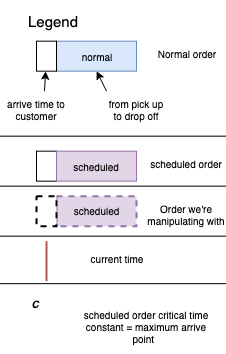
\includegraphics[scale=0.7]{orders/legend.png}
	\caption{Order planning scheme legend}\label{order-planning-legend}
\end{figure} 



\subsection{Add order}
We distinguish two main categories of added orders - scheduled order and normal (not scheduled) order. At first we have to define who can be assigned the order, and then we have to define how to do it.

Order can be assigned to either all of the available drivers or to the one specific driver. By available driver we mean the driver who is on shift and is not in pause status. Then from this set of drivers we choose the driver whom the order will be assigned to.

As mentioned before, scheduler must ensure that if the scheduled order is assigned to the driver, it is able to get there right on the pick-up time. Here appears a problem we must solve - how to count the arrive time for a given driver to that pick-up location so we can let know the driver when to start processing the order?

First naive solution lead us to count the arrive time in the moment of adding to queue. In this point we know the last order finish location, so we could count arrive time from that point. The problem is that the order we are adding can (and probably will) be week or two after the time of arrive to that location. In order to persist the calculated arrive time we have to options. First one is to forbid adding new orders before the scheduled order - that is obviously unacceptable. Second one is to during the insertion of some other order in between the last order in queue and our scheduled order count two arrive times - the newly inserted one and the scheduled one \ref{scheduled_naive_arrive_counting}. 

\begin{figure}[h]\centering
	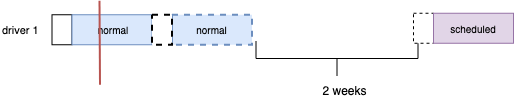
\includegraphics[scale=0.7	]{orders/scheduled_naive_arrive_counting.png}
	\caption{Scheduled order - naive arrive time calculating approach} 
	\label{scheduled_naive_arrive_counting}
\end{figure} 

Each route calculation is expensive and this naive approach doubles the costs of each processed order by the driver who has some scheduled order in the queue. Because these orders with two weeks ahead pick-up time are the most common use case in our taxi company we want to avoid this extra cost. 

We observed that there must be some point, when the arrive time of scheduled order must be calculated. If we calculate to early, we raise the costs per order. In the other case if we calculate to late the driver could not be able to get to the pick-up location on time. 

Our solution combines these two cases. Based on that observation we define the critical time constant \textit{C}. Value of this constant is equal to the maximum arrive time to any location operated by the taxi company. 

In our scheduling system then holds that each scheduled order in queue which has pick-up time less than \textit{C} from the order before it or the current time, has calculated arrive time which we update with each change. If the distance between two orders is larger than \textit{C} we do not count the arrive time.

This led to split the problem of adding order into seven parts:
\begin{itemize}
	\item Normal order - counting arrive time
	\item Normal order - selecting driver
	\item Scheduled order - counting arrive time
	\item Scheduled order - combined with other scheduled
	\item Scheduled order - combined with normal order
	\item Normal order combined with scheduled
	\item Scheduled order - scheduling on critical time callback 
\end{itemize}

	\subsubsection{Normal order - counting arrive time}
	
	First we focus on how to count the arrive time for the normal order. As we can see in \ref{order-process-normal-order-counting-arrive} there are three states in which can queue be.
	
	As in situation \textit{1a)} if the last order in queue is a normal order, calculate the arrive time as time between the finish location of that order and start of the new order.
	
	In case that the queue is empty as in \textit{1b)} calculate the arrive time as time between the last known location + time for response to the order for the driver.
	
	Third possible situation \textit{1c)} occurs when there is ongoing scheduled order. Then count arrive time as the time between finish location of that order and start of the new order.
	
	
		\begin{figure}[h]\centering
			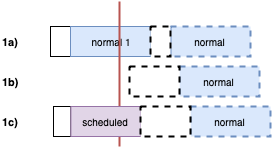
\includegraphics[scale=0.7	]{orders/add-1.png}
			\caption{Normal order - counting arrive} 
			\label{order-process-normal-order-counting-arrive}
		\end{figure} 
	
	\subsubsection{Normal order - selecting driver}
	
		As described in specification, normal order must be always assign to the driver who can pick up the customer first. This rule demonstrates the example  \ref{order-process-normal-order-selecting-driver}. The order will be assigned to the \textit{driver 1} even though the \textit{driver 2} is available first.
			
			\begin{figure}[h]\centering
				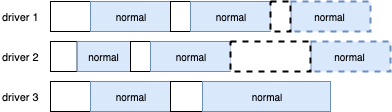
\includegraphics[scale=0.7	]{orders/add-2.png}
				\caption{Normal order - counting arrive} 
				\label{order-process-normal-order-selecting-driver}
			\end{figure} 
		
	\subsubsection{Scheduled order - counting arrive time}
		If we add scheduled order to the driver's queue in which there is no other order within the critical time constant, we do not calculate the arrive time of that order\ref{order-process-scheduled-order-counting-arrive-time}. We are allowed to do so, because the critical time constant \textit{C} ensures, that if the queue stayed in the same state, the arrive time between the last location to the order start will be less than \textit{C}.
		
		\begin{figure}[h]\centering
			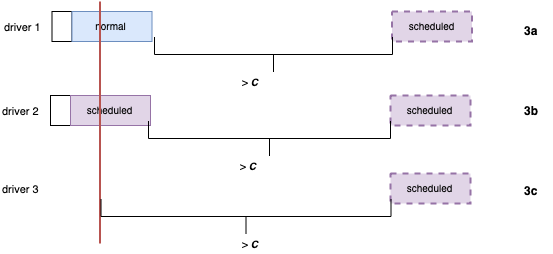
\includegraphics[scale=0.7	]{orders/add-3.png}
			\caption{Scheduled order - counting arrive time} 
			\label{order-process-scheduled-order-counting-arrive-time}
		\end{figure} 
	
	
	\subsubsection{Scheduled order - combined with other scheduled}
			In case that the scheduled order has other scheduled order within \textit{C} from the calculated pick-up and finish time, we have to calculate corresponding arrive times \ref{order-process-scheduled-order-combined-with-scheduled}. 
			After the calculation we may encounter the orders collision. In such case the order can not be added to the queue and the order scheduler must throw an error. 
			
			\begin{figure}[h]\centering
				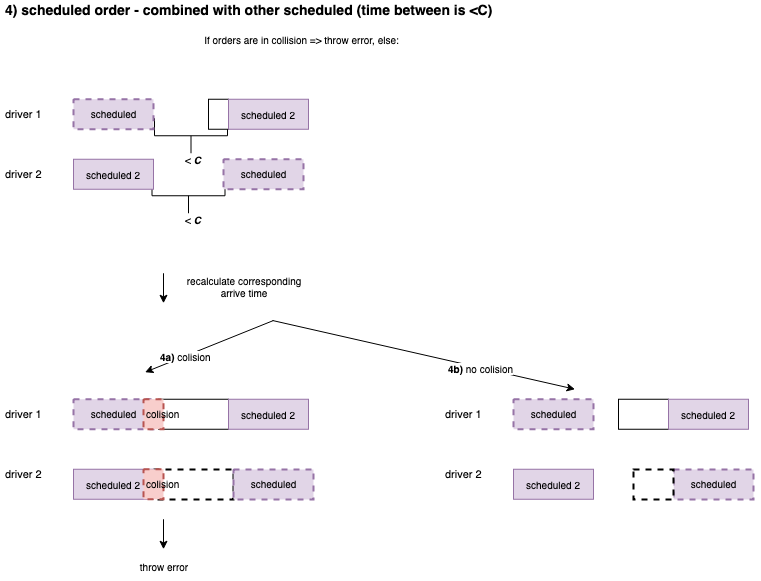
\includegraphics[scale=0.6	]{orders/add-4.png}
				\caption{Scheduled order - combined with other scheduled} 
				\label{order-process-scheduled-order-combined-with-scheduled}
			\end{figure} 
		
	\subsubsection{Scheduled order - combined with normal order}
		When the expected finish time is within the \textit{C} from the inserted scheduled pick-up time, we must calculate the arrive time. In case that the the scheduled order is in collision with some normal order, scheduler must throw an error \ref{order-process-scheduled-order-combined-with-normal}.
		 
		\begin{figure}[h]\centering
			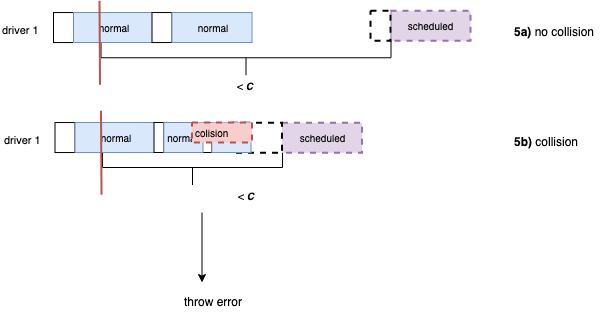
\includegraphics[scale=0.6	]{orders/add-5.png}
			\caption{Scheduled order - combined with normal order} 
			\label{order-process-scheduled-order-combined-with-normal}
		\end{figure} 
	
			
	\subsubsection{Normal order - combined with scheduled}
	Adding new normal order to queue could break the fact that each of the scheduled orders in our system has counted arrive time if the pick-up time is at least \textit{C} from the finish time of order before it.
	
	If this situation occurs, we must recalculate the arriving time of the scheduled order after it -  accordingly with respect to the new finish location. This change can lead to collision. In case we encounter the collision, we start the process of adding the order again. In this second try we consider as the previously picked queue's finish location the finish location of collided scheduled order. Also the arrive time of the colliding scheduled order must be set back to the original value. 
	 \ref{order-process-normal-order-combined-with-scheduled}.
	
	\begin{figure}[h]\centering
		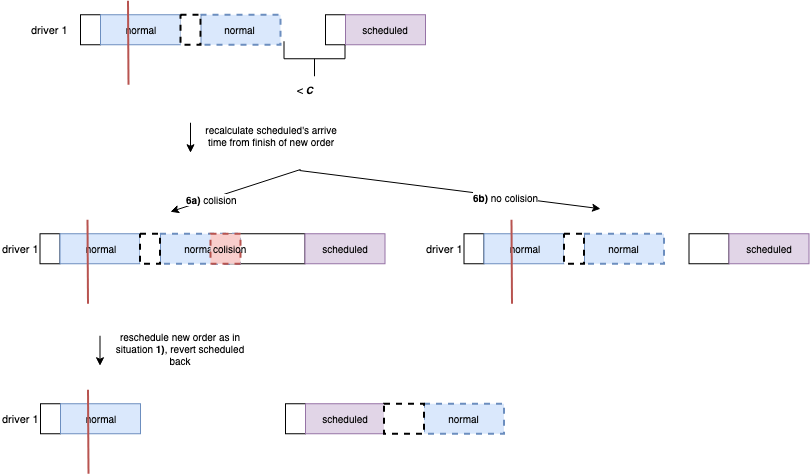
\includegraphics[scale=0.5	]{orders/add-6.png}
		\caption{Normal order - combined with scheduled order} 
		\label{order-process-normal-order-combined-with-scheduled}
	\end{figure} 

	\subsubsection{Scheduled order - scheduling on critical time callback}
	As we know scheduled orders have not calculated arriving time when their pick-up time is within \textit{C} from any other order finish in queue or the current time. In previous cases we described all the possible situations how can order be added before the scheduled order within the time constant. Last thing we have to cover is the situation when the current time exceeds a point from which is the the pick-up time of our order less than C.
	
	This situation we would cover with callback which is called exactly in that point. If the order does not have arrive time calculated in that point, we calculate it from the last known drivers location and the order start location. 
	 \ref{order-process-scheduled-critical-time}.

	\begin{figure}[h]\centering
		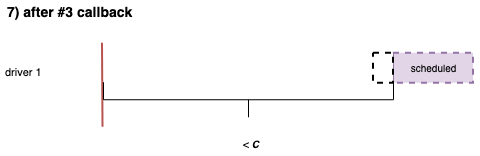
\includegraphics[scale=0.7]{orders/add-7.png}
		\caption{Scheduled order - critical time callback} 
		\label{order-process-scheduled-critical-time}
	\end{figure} 

\subsection{Change arrive time}
	Estimated order times can be manually changed by driver during the order. Average expected time change in such cases is within a few minutes. We can divide the change of time into two groups. In the first one the order will take longer after the change, in the second one the order will be shorter.
	
	\subsubsection{Longer order}
	When the order takes longer than it was expected to we just take all the normal orders after it until the first scheduled one and we move their start times accordingly\ref{order-process-change_longer}.
	\begin{figure}[h]\centering
		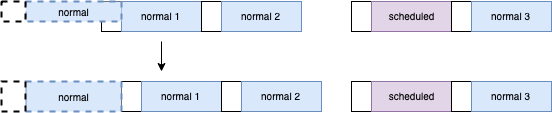
\includegraphics[scale=0.7]{orders/changing_arrive_time_longer.png}
		\caption{Change arrive time - longer order} 
		\label{order-process-change_longer}
	\end{figure} 

	During this change there can occur collision with some scheduled order in queue. If the colliding order is normal order, we reschedule it the same way as we were adding it \ref{order-process-change_collision_normal}. 
	
	\begin{figure}[h]\centering
		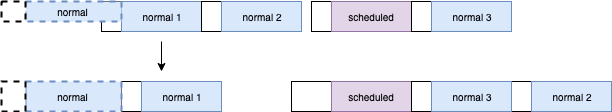
\includegraphics[scale=0.65]{orders/changing_arrive_time_longer_normal_collision.png}
		\caption{Change arrive time - longer order - collision of normal and scheduled order} 
		\label{order-process-change_collision_normal}
	\end{figure} 

	If the collision is between scheduled or ongoing order, we must shift the start of the following scheduled order \ref{order-process-change_collision_scheduled}.
	
	\begin{figure}[h]\centering
		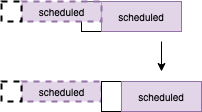
\includegraphics[scale=0.7]{orders/changing_arrive_time_longer_scheduled_collision.png}
		\caption{Change arrive time - longer order - collision of two scheduled orders} 
		\label{order-process-change_collision_scheduled}
	\end{figure} 
	
	
	\subsubsection{Shorter order}
		When the time change makes the order shorter, we just simply change the starting time estimation accordingly for all of the normal orders after it until the first scheduled one
		\ref{order-process-change-shorter}.
		
		\begin{figure}[h]\centering
			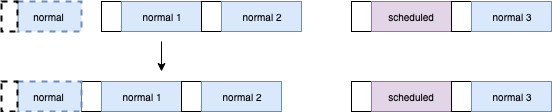
\includegraphics[scale=0.7]{orders/Shorter_order.png}
			\caption{Change arrive time - shorter order} 
			\label{order-process-change-shorter}
		\end{figure} 
	
\subsection{Cancel}
	When the order is cancelled, we must remove it from the driver's queue and reschedule each order after the cancelled order - except the scheduled one. By rescheduling we mean sequence of two actions - cancel and add \ref{order-process-cancel}.
	
	\begin{figure}[h]\centering
		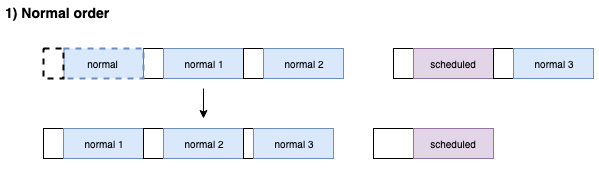
\includegraphics[scale=0.7]{orders/cancel.png}
		\caption{Cancel the order} 
		\label{order-process-cancel}
	\end{figure} 
	We suppose that the order cancel is rarely called, so we do not pressure on the route calculation optimization as much.

\subsection{Change driver}
Changing the driver should happen even less than cancelling the order. In such case it is sufficient just to call the \textit{cancel} action and \textit{add} action with the specified selected driver.
	 